\capitulo{5}{Aspectos relevantes del desarrollo del proyecto}

Este apartado pretende recoger los aspectos más interesantes del desarrollo del proyecto, la exposición del ciclo de vida, y detalles de mayor relevancia en las fases de análisis, diseño e implementación.

\section{Inicio del proyecto}


En una primera reunión se realizó una primera  discusión sobre el artículo \cite{problemn-alkanes2007}, para entender los objetivos reales del proyecto. 

A partir de este momento se buscaron opciones para llevar a cabo el desarrollo de una web que realizara operaciones de programación lineal para calcular las composiciones de la dieta de grupos de animales (más adelante se entendió que realmente  esta implementación  permitía resolver otros muchos problemas dentro del marco de los \emph{Mixing Models}). Las dos grandes alternativas a la hora de desarrollar la web fueron React vs Angular.

\section{Selección React vs Angular}

Con el objetivo de ordenar y aclarar diferencias entre React y Angular se ha realizado la tabla \ref{tab:reactvsangular}.

\begin{table}[h]
    \centering
    \begin{tabular}{| m{2.5cm} | m{5cm} | m{5cm} |}
    \hline
        Característica & React & Angular \\ \hline
        ¿Que es? & Javascript framework & Javascript biblioteca para el desarrollo de interfaces gráficas \\ \hline
        Tipo de Webs & Web y móvil, Single- y Multiple-page applications & Web y móvil, Single- y Multiple-page  applications\\ \hline
        Aprendizaje & Largo y difícil & Rápido y simple si se conoce Javascript previamente\\ \hline
        Comunidad & Grande & Grande\\ \hline
        Rendimiento & Optimizado con detección de cambios & Optimizado con virtual DOM\\ \hline
        Lenguajes & JavaScript, TypepScript & JS ES6+, JSX script\\ \hline
        Estructura de la APP & Fijo y complejo, componentes basados en MVC & Flexible, componentes  basados en vistas\\ \hline
        Directivas & Incomprensibles sin conocimiento previo en Angular & Fáciles de entender con conocimiento en Javascript\\ \hline
        Vinculación de datos & Bidireccional, datos mutables & Unidireccional, datos  inmutables\\ \hline
        Herramientas & Aptana, Sublime Text, Visual Studio, Angular CLI, Angular Universal, Jasmine,  Protractor, Karma & Sublime Text, Visual Studio, Atom, Create React App (CLI), Next.js framework, Enzyme, Hest, React-unit\\ \hline
        Añadir librerias en Javascript en el código & Posible & No posible\\ \hline
    \end{tabular}
    \caption{Comparativa entre React y Angular. Fuente: Elaboración propia}
    \label{tab:reactvsangular}
\end{table}

\newpage

Inicialmente, el lenguaje más atractivo era React por su facilidad de aprendizaje y uso.
Un punto que nos preocupaba tanto a mí como a los tutores en cuanto al diseño de la web, era que fuera Single-page-application, opción que permiten los dos lenguajes. 
Por parte de los lenguajes de programación, se partía de cero en los dos casos, al yo no tener conocimientos previos en Javascript ni en Typescript.
En cuanto a la estructura de la APP, el MVC ha sido estudiado en algunas asignaturas durante la carrera, habiéndole dado más importancia que modelos basados únicamente en vistas.
Respecto a las herramientas, se conocían con anterioridad Sublime Text y Visual Studio, que son comunes en los dos lenguajes y no tienen una gran importancia en cuanto al uso exclusivo de un lenguaje, al ser los dos editores de textos.

En este caso, hubo un punto más a tener en cuenta, y es que durante este año he estado realizando prácticas en una empresa, y el lenguaje con el que se ha trabajado ha sido Angular, de modo que para reducir tiempos de formación y trabajar en un lenguaje un poco más conocido se decidió seleccionar Angular como el lenguaje principal para el desarrollo del proyecto al no tener previamente una mayor diferenciación a parte de su simplicidad de aprendizaje por parte de React.

\section{Metodología}

La metodología utilizada ha sido SCRUM, metodología aprendida en la asignatura de \emph{Gestión de Proyectos}. SCRUM es un marco de trabajo para desarrollo ágil, el cual son un conjunto de buenas prácticas para trabajar de forma colaborativa y obtener el mejor resultado  posible.

Algunas de las medidas características de la metodología que se han aplicado en el proceso de desarrollo son:

\begin{itemize}
	\item La  planificación del desarrollo se ha realizado en periodos de una misma duración con objetivos claros, llamados \emph{"sprints"}. Estos se encuentran en el repositorio de GitHub \url{https://github.com/humbertoms99/DIET_COMPOSITION}.
	\item El desarrollo  de la aplicación ha sido incremental.
	\item Se han mantenido reuniones al final de cada sprint para hablar de las implementaciones y próximos desarrollos. 
	\item Se ha estimado el valor de los objetivos de los \emph{sprints}  mediante Story points. 
	\item Se han añadido, movido y completado tareas mediante la herramienta Zenhub.
	\item Se ha establecido un tiempo de 2 semanas por cada sprint.
\end{itemize}

\section{Desarrollo del proyecto}

Durante las primeras semanas se realizó un curso de \LaTeX{} \cite{curso:latex}, con el objetivo de documentar las elecciones entre herramientas. 

Posteriormente  se pasó a documentar el problema planteado en el articulo \cite{problemn-alkanes2007} sobre el problema de n-alcanos, siendo el objetivo inicial del proyecto.

Uno de los objetivos más importantes para el funcionamiento del proyecto fue el uso de una biblioteca que resolviera problemas de programación lineal, como \cite{glpk:package}. El proceso de instalación y configuración de esta biblioteca conllevó algunos problemas: el primer problema fue la necesidad de ejecutar algunos comandos de la instalación desde una terminal Linux. Al estar trabajando en un entorno Windows se decidió continuar en el sistema operativo,  por lo que se optó  por usar una herramienta que actuara como subsistema  Linux en Windows 10, en este caso Debian \cite{debian}, al ser este un software gratuito y con distribución libre.

Otro problema que surgió durante la configuración de la librería fue el requerimiento de un compilador en C, ya que la librería está escrita en ANSI C, lo cual se resolvió con siguiendo los pasos de una respuesta encontrada en StackOverFlow \cite{stack:Compiler}. Otro punto a destacar sobre el uso de esta librería, es que requiere  que el servidor se este ejecutando en una terminal Linux, por lo que se configuró Visual Studio Code para escribir comandos en una terminal Linux.

Una vez entendidos los objetivos del problema a resolver y disponer de una librería que resolviera estos requerimientos, comenzó la fase  de implementación, dividiendo esta parte del desarrollo en periodos muchos más marcados con requisitos claros y trabajando simultáneamente en el proyecto front-end en Angular y el back-end en un proyecto laravel. A continuación analizaremos algunos de los puntos que consideramos claves de implementación.

\subsection{Formularios}

Angular ofrece dos técnicas para crear formularios: formularios basados en plantillas (Template Forms) y formularios reactivos (Reactive Forms). 

Se optó por realizar los formularios  reactivos, al ser más sencillos, ya que las validaciones se trabajan desde la clase componente siendo  una lógica más limpia, al pasar las validaciones al componente. Al contrario que los formularios por plantilla, es más fácil definir formularios dinámicos (punto importante al trabajar con una matriz que va cambiar de tamaño).

La diferencia principal es que los \emph{Reactive Forms} definen el formulario en la clase del componente y trabajan  en la vista con las directivas \emph{formGroup} o \emph{formControlName},  al contrario que los \emph{Template Forms}, donde las reglas y estructura del  formulario se hacen en la vista utilizando directivas como \emph{ngForm} y \emph{ngModel}

Para mantener la idea de separación entre vista y lógica, se decidió utilizar los \emph{Reactive Forms}, que además son más fáciles de usar y permiten más adaptaciones por parte de las validaciones.

\begin{figure}[h!] 
\centering
    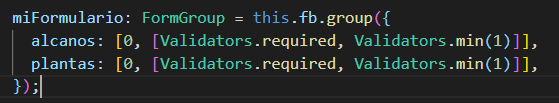
\includegraphics[width=0.8\textwidth]{img/formIndexMatrix.PNG}
\caption{Fórmulario index Matrices}
\label{fig:formIndexMatrix}
\end{figure}

En la figura \ref{fig:formIndexMatrix} se puede ver el código de clase del componente que contendrá los índices de la matriz de datos a solicitar posteriormente. Estos campos son siempre requeridos y deben tener un valor superior a "1"; por el contrario, el botón de crear matrices permanecerá deshabilitado.

\begin{figure}[h!] 
\centering
    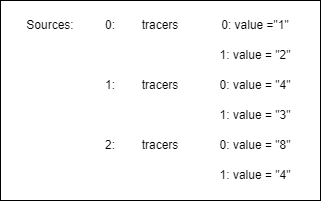
\includegraphics[width=0.8\textwidth]{img/formSources.png}
\caption{Estructura de datos del formulario que contiene los valores de las fuentes}
\label{fig:formSources}
\end{figure}

En la Figura \ref{fig:formSources} podemos observar la estructura del segundo formulario que contendrá los datos de la matriz de datos con los valores de los marcadores para cada fuente. La estructura de este formulario es un "\textit{array de Sources}"  que tendrá tantos elementos como fuentes se especifiquen en los \textit{index} del anterior formulario. Cada elemento está formado por un único \textit{formArray} de marcadores (tantos como se especificaron en el primer formulario). En este último array se encuentran los correspondientes valores de cada marcador para la fuente.

\begin{figure}[h!] 
\centering
    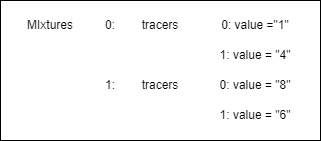
\includegraphics[width=0.8\textwidth]{img/formMixtures.png}
\caption{Estructura de datos del formulario que contiene los valores de las mezclas}
\label{fig:formMixtures}
\end{figure}

En la Figura \ref{fig:formMixtures}  observamos la estructura de datos del tercer formulario que contiene los datos de las mezclas sobre las cuales queremos calcular el problema. Estos datos son rellenados mediante la interfaz al usar el botón de añadir mezcla. La estructura del formulario es un "\textit{array de Mixtures}"  que tendrá tantos elementos como mezclas se crean en la interfaz. Cada elemento esta formado por un único \textit{formArray} de marcadores (tantos como se especificaron en el primer formulario). En este último array se encuentran los correspondientes valores de cada marcador para la fuente.

Por último, se implementó un cuarto formulario que permite  el cambio de nombre de las fuentes, con el objetivo de hacer más visible las posibilidades de resolver el problema de los \textit{Mixing Models}.

\subsection{Estructura documentos csv}

En esta sección visualizaremos los archivos .csv exportados por la aplicación web y  explicaremos su estructura.

\subsubsection{Export Input Data}

En la Figura \ref{fig:inputData} podemos ver una vista de los datos que corresponden al archivo \textit{InputData.csv}; este archivo será el esperado en la opción de importar datos.

Las dos primeras filas marcan el número de marcadores y fuentes  respectivamente. A continuación, siempre se dejará una línea vacía que marca que las siguientes líneas son los valores para cada fuente; el número de filas de fuentes corresponderá al número de fuentes fijado en la segunda fila. Para diferenciar las filas referentes a los valores de las mezclas  se deja otra fila vacía. Es obligatorio dejar estas filas vacías para que la entrada de los datos sea correcta.

\begin{figure}[h!] 
\centering
    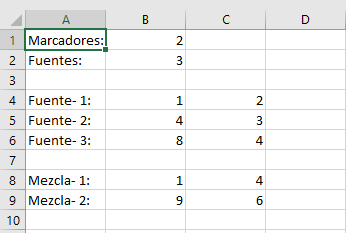
\includegraphics[width=0.8\textwidth]{img/inputData.PNG}
\caption{Vista csv InputData}
\label{fig:inputData}
\end{figure}

\subsubsection{Export Solution}

En la figura \ref{fig:solution} podemos ver la vista de  la solución del problema. Se ha intentado que mantuviera una disposición similar a la de la aplicación web. En una primera parte tenemos los datos del problema tal cual se encuentran en el archivo \textit{InputData.csv}. Posteriormente se añade una línea con la proyección de la muestra usada para realizar el calculo.

Por último, podemos  apreciar una estructura de tabla en la cual podemos ver las estimaciones máximas y mínimas de las mezclas sobre las fuentes.

\begin{figure}[h!] 
\centering
    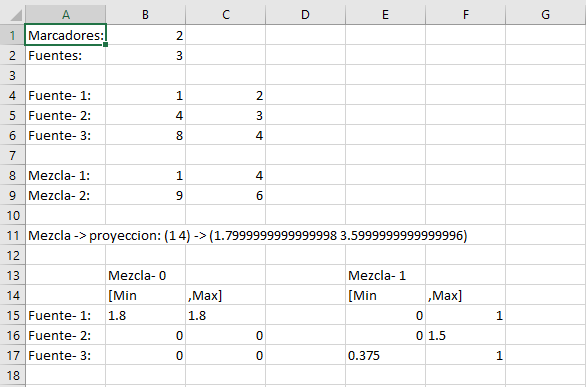
\includegraphics[width=0.8\textwidth]{img/solution.PNG}
\caption{Vista csv Solution}
\label{fig:solution}
\end{figure}

\subsubsection{Export Paso Intermedio }

En el caso de los dos tipos de exports vistos previamente, la descarga era trivial  ya que se mostraban sus pertinentes botones de exports una vez realizado el cálculo. En el caso de que queramos ver los cálculos intermedios realizados para cada valor, sera necesario dar click sobre el propio valor de estimación tanto para máximos, que descargará un archivo con nombre \textit{M1\_max1.csv}, como para mínimos, donde el fichero se llamará \textit{M1\_min1.csv}. El nombre es una simplificación de "Mixture 1 - Maximize Source 1".

El contenido de la Figura \ref{fig:pasoIntermedio} corresponde con los archivos \textit{.mod} usados desde la API para resolver el problema de maximización de un objetivo sobre un conjunto de reglas y ecuaciones. La segunda columna  marca el tipo de línea que es, teniendo líneas para la definición de las variables: una  única línea que señaliza el tipo de operación (maximización o minimización) y la función objetivo, y unas últimas líneas que contendrán las ecuaciones con los índices de los marcadores tanto para fuentes como para las mezclas

\begin{figure}[h!] 
\centering
    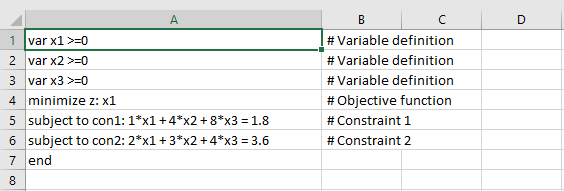
\includegraphics[width=0.8\textwidth]{img/pasoIntermedio.PNG}
\caption{Vista csv paso intermedio}
\label{fig:pasoIntermedio}
\end{figure}

\newpage
\section{Ciclo de la aplicación}

En este apartado vamos a comentar los pasos que realiza la aplicación y nos detendremos en los que consideremos más importantes

Al entrar a la web en la parte superior veremos un \textit{"Top Navigation Bar"} \cite{Navigation:Bar}, donde la primera ventana ha sido dedicada a la resolución del problema, una segunda con un vídeo guía de uso de la aplicación, el icono con enlace directo al GitHub y finalmente un apartado de las personas participantes en el desarrollo del proyecto.
Justo debajo encontraremos el primer formulario con dos inputs para introducir los índices de la matriz de fuentes. junto con dos botones:  botón \textit{``Crear''} y  \textit{"Seleccionar archivo"}. Este segundo lanza un evento y permite leer archivos con el formato esperado.

Estos dos botones marcan las dos alternativas del flujo en la Figura \ref{fig:cicloDeVida}. En el caso de la rama izquierda del flujo  (\textit{``Introducción manual de los datos''}) es necesario rellenar el primer formulario con los índices, un segundo con los valores de las fuentes y dar valores para las mezclas (pudiendo añadir más mezclas con su botón correspondiente).

Estos dos flujos se unen al dar al botón \textit{``Resolver''}. Al hacer click se calcularán las proyecciones de las mezclas, y en caso de ser diferentes a las mezclas originales se mostrará un mensaje en pantalla con los valores sobre los que se han realizado los cálculos. 



\begin{figure}[h!] 
\centering
    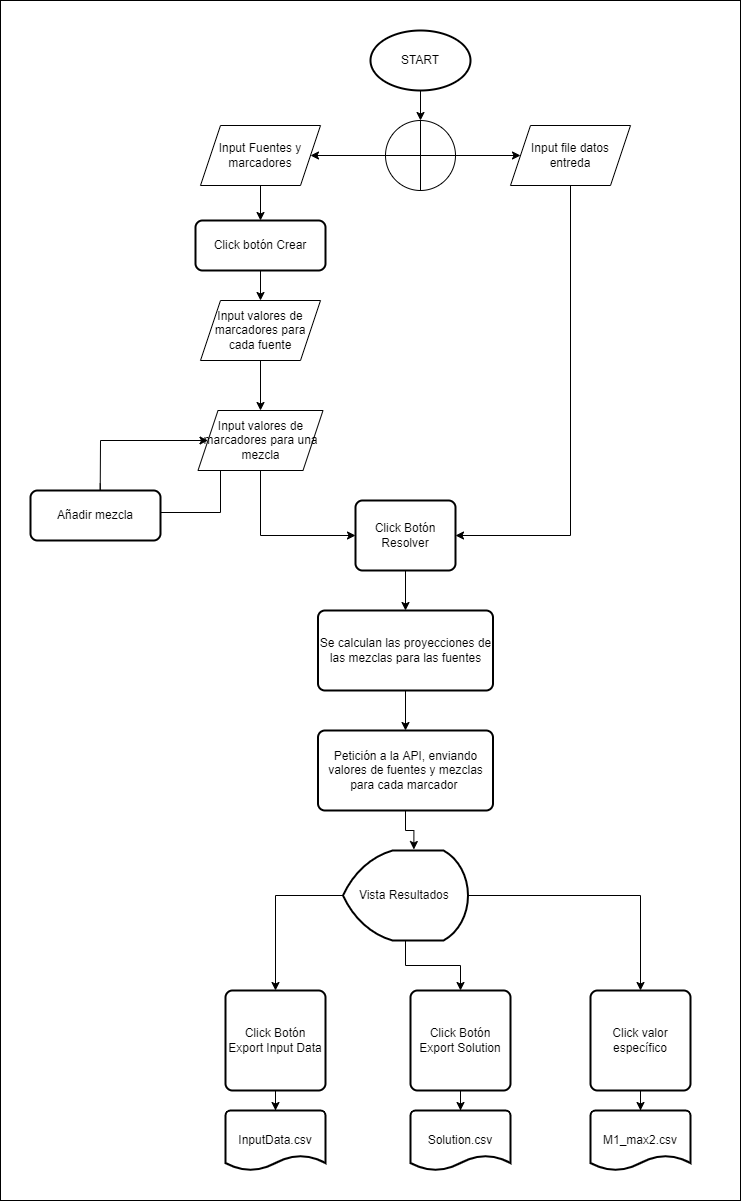
\includegraphics[width=0.8\textwidth]{img/cicloDeVida.png}
\caption{Ciclo de vida }
\label{fig:cicloDeVida}
\end{figure}

Una vez se han calculado las proyecciones de las mezclas, se ejecuta una petición por cada mezcla con los arrays de fuentes y valores para la mezcla al API. Esta petición genera un archivo tipo \textit{"file\_max1\_1.mod"} en la ruta \textbf{storage/app} del  proyecto en laravel por cada marcador que tiene cada mezcla. Su contenido es equivalente al mostrado en la figura \ref{fig:pasoIntermedio}. Para resolver el problema de maximización o minimización, hacemos uso de la librería \cite{glpk:package} con el comando \textit{"glpsol -m ../storage/app/file\_max1\_1.mod -o files\_sol/file\_max1\_1.sol"} que nos genera un archivo tipo \textit{".sol"}. Este comando requiere  ser ejecutado desde una terminal Linux (En el entorno local se uso debian wsl \cite{debian}); este comando genera un archivo tipo \textit{".sol"} en la ruta \textit{public/files\_sol/}.

\begin{figure}[h!] 
\centering
    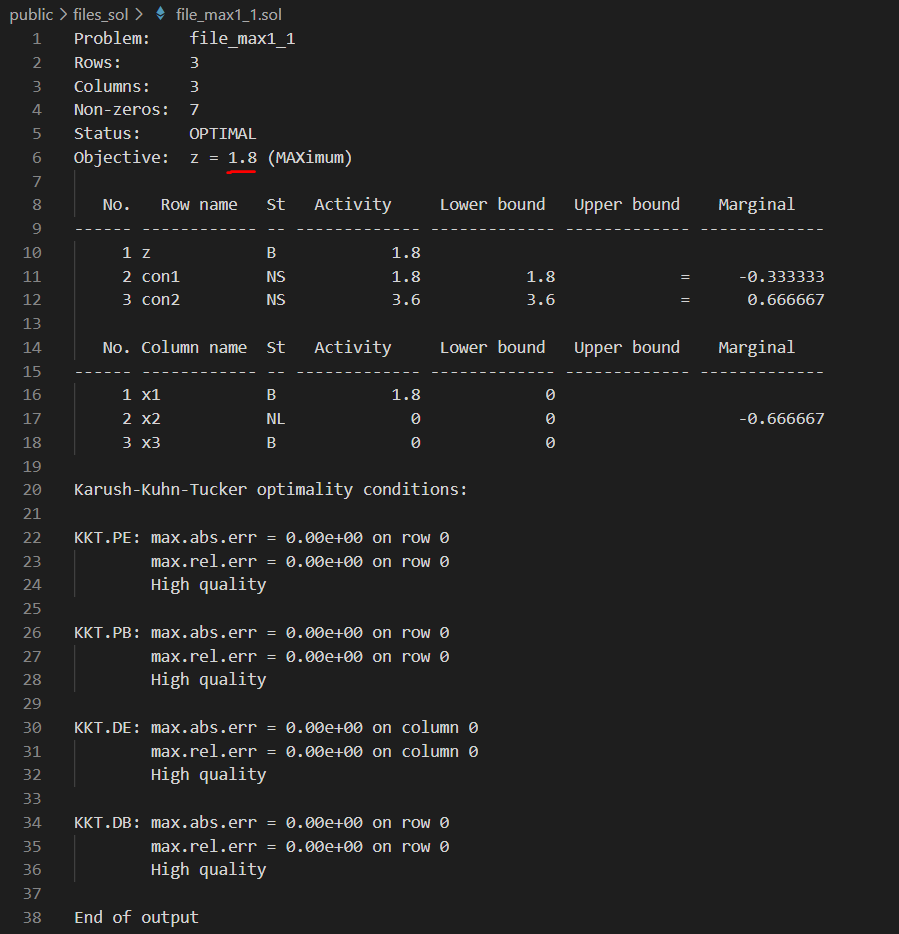
\includegraphics[width=0.8\textwidth]{img/fileSol.PNG}
\caption{Archivo file\_max1\_1.sol }
\label{fig:fileSol}
\end{figure}

Dicho archivo, denominado \textit{file\_max1\_1.sol}, devuelve el valor objetivo calculado en la línea $6$, como podemos ver en la figura \ref{fig:fileSol}. El método agrupará los objetivos de todos los archivos generados en arrays de máximos y mínimos por mezcla y se retornan como repuesta JSON (Figura \ref{fig:respuestaJson}).

\begin{figure}[h!] 
\centering
    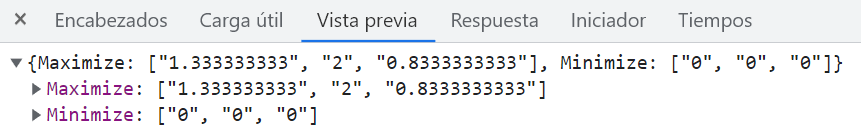
\includegraphics[width=1\textwidth]{img/respuestaJsonMax.PNG}
\caption{Respuesta JSON formado los arrays máximos y mínimos de una mezcla. }
\label{fig:respuestaJson}
\end{figure}

Por último, se muestra en la web los resultados de los cálculos junto con los botones de exportación de los datos de entrada y de la solución. 

\section{Problema subida API a Heroku}

Inicialmente se desarrolló el proyecto en dos códigos: una API que utilizaba la librería GLPK escrita en C y una parte front que se comunicaba con esta API mediante peticiones. Estos dos proyectos se desarrollaron por completo, funcionando ambos correctamente en un entorno local.

Uno de los requisitos del proyecto es que fuera una herramienta accesible, y que se desplegara como aplicación web. Por este motivo se seleccionaron Heroku para subir el proyecto back-end y Netlify para el proyecto front-end. Los códigos se consiguieron subir sin problemas. Pero en el caso de la API, necesitaba contar con la librería GLPK instalada en el servidor.  La librería GLPK usada en el entorno local no se consiguió instalara en un servidor web gratuito. 

Por este motivo, se tomó la decisión de cambiar el código front-end ya subido a producción, haciendo que el proyecto front-end en Angular, no necesitara el uso de la API. En este momento se realizó una búsqueda de librerías que pudieran ejecutarse en Typescript y resolvieran los mismos problemas que  el paquete GLPK. Las opciones finales fueron: \url{https://www.npmjs.com/package/glpk-ts} y \url{https://www.npmjs.com/package/glpk.js}. Finalmente, y ya que la lógica del código está desarrollada en Typescript se instaló y aprendió a utilizar \textbf{glpk-ts}. Este paquete es una interfaz de la misma librería GLPK \cite{glpk:package} que se usa desde módulos. 

Este cambio ha significado no realizar peticiones a la API, lo cual ha derivado en un desarrollo de estas funcionalidades en el proyecto front-end. 

\section{Internacionalización}

A través de la internacionalización se consigue realizar un proceso de expansión del software. Se ha diseñado la aplicación permitiendo intercambiar entre diferentes idiomas. Se proporcionan dos idiomas: Español e Inglés. Esto se permite desde una select en el menú superior que está siempre visible (figura \ref{fig:selectidiom}), cambiando este valor se lanza un evento que cambia una variable en el localStorage. Esta variable marca el fichero de traducciones a tomar por la aplicación. Los ficheros de traducciones se encuentran en la ruta \textbf{src/assets/i18n} y tienen extensión .json.

\begin{figure}[h!] 
\centering
    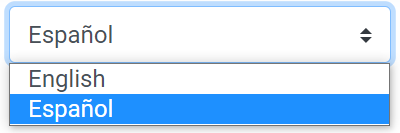
\includegraphics[width=0.8\textwidth]{img/selectIdiom.PNG}
\caption{Select de Idioma}
\label{fig:selectidiom}
\end{figure}

\newpage
Para realizar traducciones desde angular se hace uso del módulo Angular Translate, que mediante el pipe \textbf{translate} marca que ese texto tiene una traducción. En la ejecución de la aplicación se carga el fichero .json correspondiente a la variable \textbf{lang} en el localStorage. La estructura de estos archivos la podemos ver en la figura \ref{fig:en_json}: consiste en una cadena de texto (línea de código escrita en el fichero \emph{.html}), el símbolo \textbf{``:''} y una cadena de la traducción al idioma correspondiente.

\begin{figure}[h!] 
\centering
    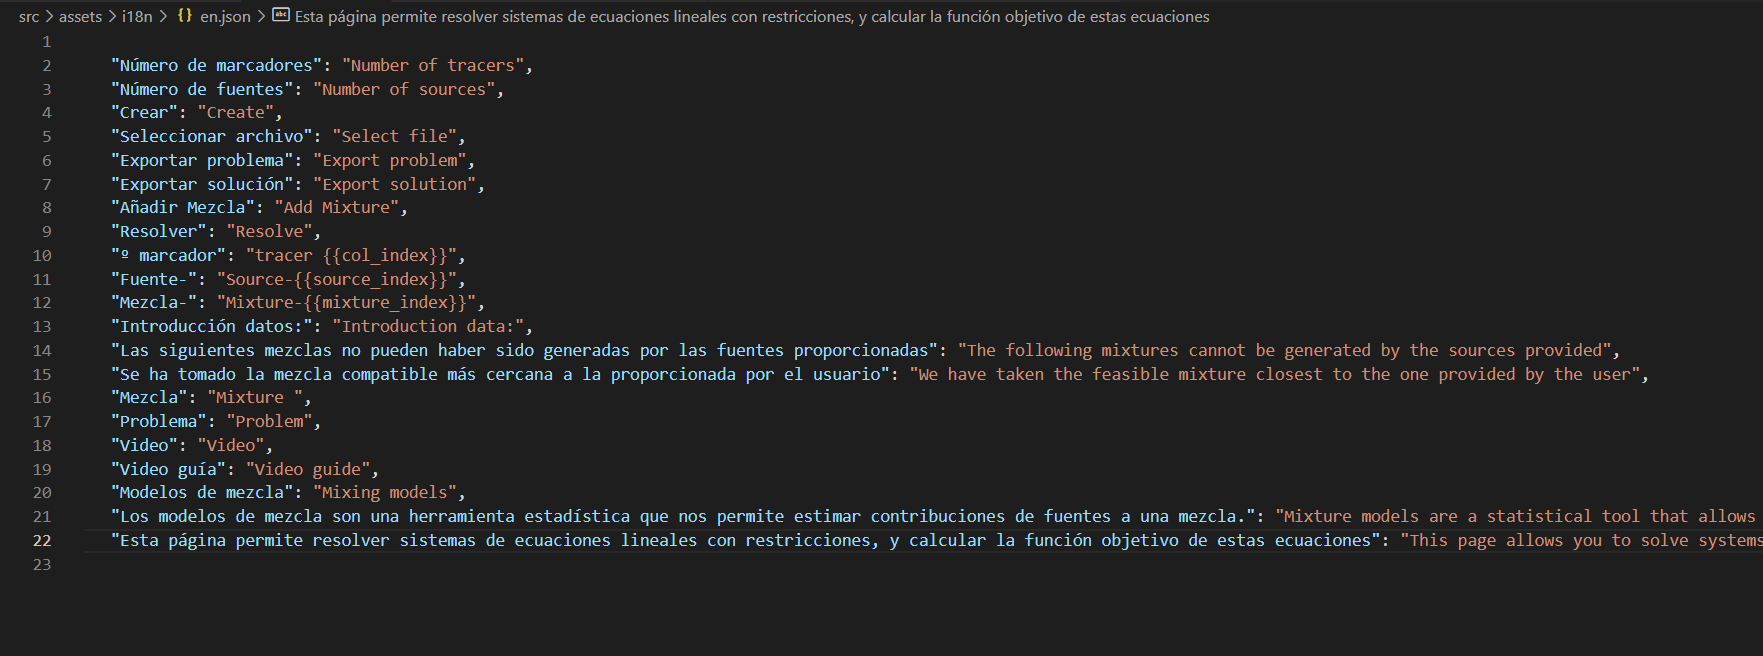
\includegraphics[width=1\textwidth]{img/en_json.PNG}
\caption{Archivo en.json}
\label{fig:en_json}
\end{figure}








